
\section{Experiments}
\label{sec:experiments}

We evaluate the main proposed methods, ECPO and ECAC,
on a number of benchmark tasks against strong baseline methods.
Implementation details are provided in the appendix. 

\begin{figure*}[t]
\begin{center}
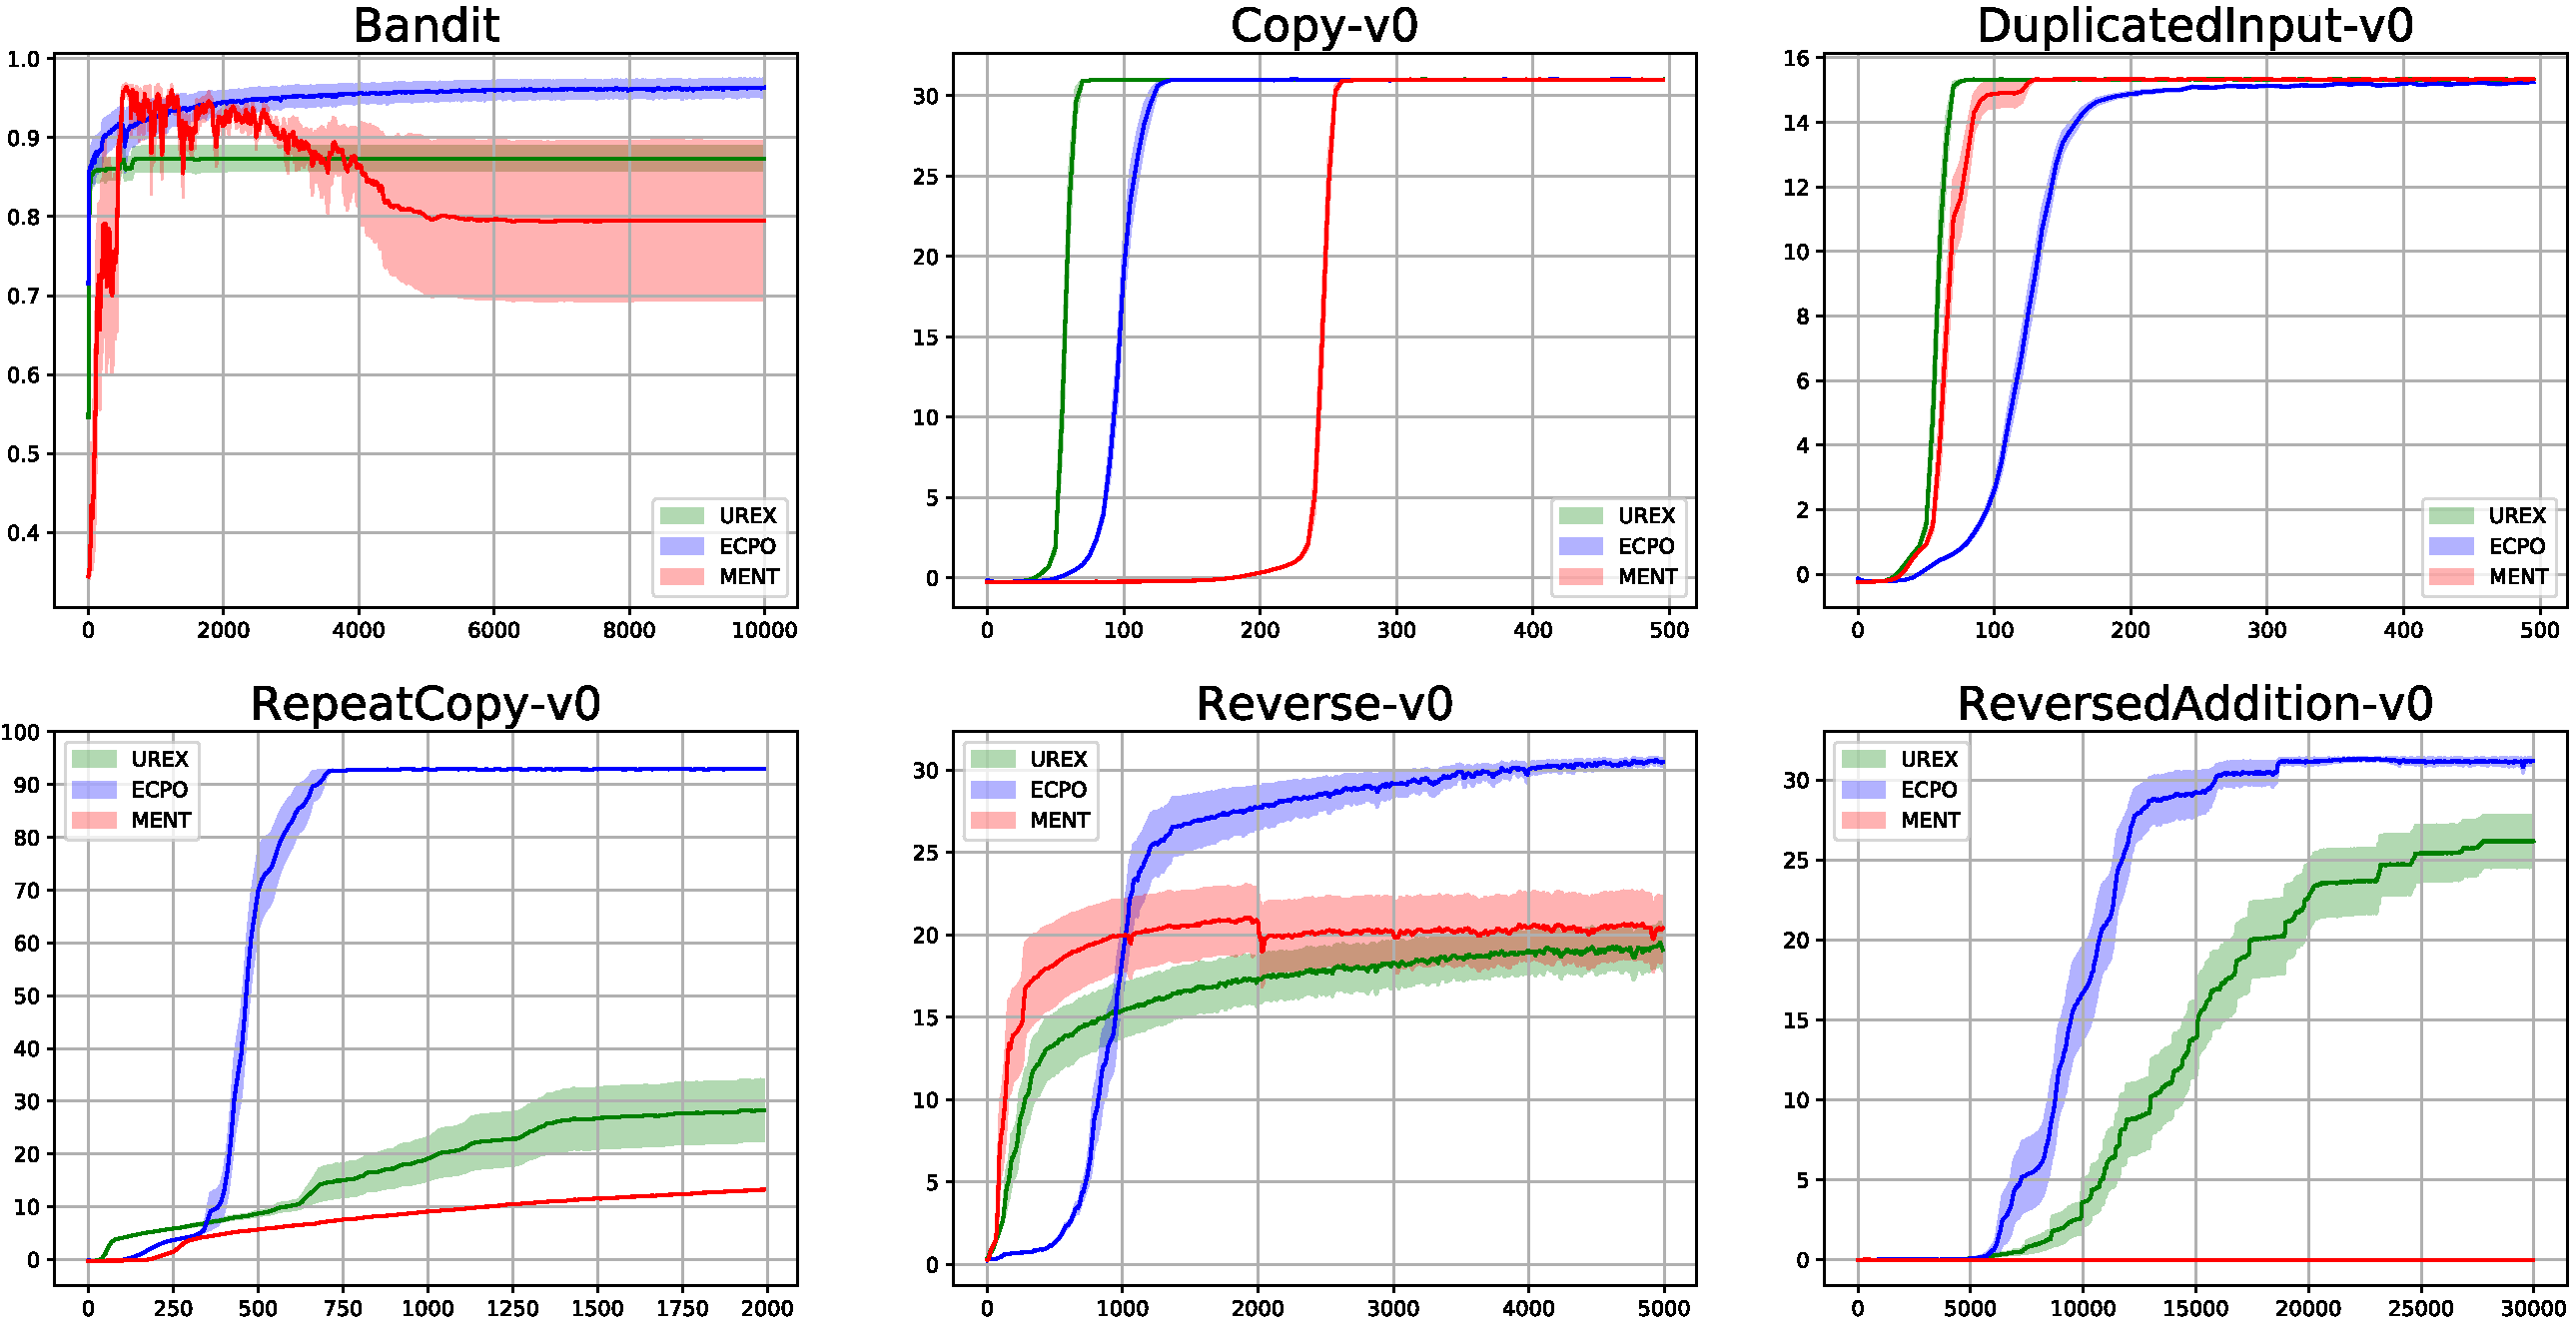
\includegraphics[width=0.7\linewidth]{./bandit_algorithmic_results.pdf}
\end{center}
\caption{
Results of MENT (red), UREX (green), and ECPO (blue) on synthetic bandit
problem and algorithmic tasks.
Plots show average reward with standard error during training.
Synthetic bandit results averaged over 5 runs.
Algorithmic task results averaged over 25 random training runs
(5 runs $\times$ 5 random seeds for neural network initialization).
X-axis is number of sampled trajectories.
} 
\label{fig:results}
\end{figure*}

\subsection{Settings}
\label{subsec:tasks}

We first investigate the performance of ECPO on a synthetic bandit problem
and the algorithmic task suite from the OpenAI gym \citep{brockman2016openai}.
The synthetic multi-armed bandit problem has $10000$ distinct actions,
where
the reward of each action $i$ is initialized by $r_i = s_i^{8}$
such that $s_i$ is randomly sampled from a uniform $[0,1)$ distribution.
Each action $i$ is represented by a randomly sampled feature vector
$\omega_i\in \mathbb{R}^{20}$ from standard normal distribution.
Note that these features are fixed during training.
We further test our method on five algorithmic tasks from the OpenAI gym
library, in rough order of difficulty:
Copy, DuplicatedInput, RepeatCopy, Reverse, and ReversedAddition
\citep{brockman2016openai}.
%
Second, we test the second ECAC approach on continuous-control benchmarks
from OpenAI Gym, utilizing the Mujoco environment
\citep{brockman2016openai,todorov2012mujoco};
including Hopper, Walker2d, HalfCheetah, Ant and Humanoid.
The details of the algorithmic and Mujoco tasks are provided in the appendix.
%\cref{subsec:benchmarks}. 

Note that only cumulative rewards are available in the
synthetic bandit and algorithmic tasks.
Therefore, value-based methods cannot be applied here, which compels us to compare ECPO against
REINFORCE with entropy regularization (MENT) \citep{williams1992simple},
and under-appreciated reward exploration (UREX) \citep{nachum2017improving}, which are state-of-the-art policy-based algorithms for the algorithmic tasks.
%
For the continuous control tasks, we compare ECAC
with deep deterministic policy gradient (DDPG) \citep{lillicrap2015continuous},
an efficient off-policy deep RL method;
twin delayed deep deterministic policy gradient algorithm (TD3)
\citep{fujimoto2018addressing},
a recent extension of DDPG by using double Q-learning;
and Soft-Actor-Critic (SAC) \citep{haarnoja2018soft},
a recent state-of-the-art off-policy algorithm on a number of benchmarks.
All of these algorithms are implemented in \emph{rlkit}.%
%
\footnote{
https://github.com/vitchyr/rlkit
}
We do not include TRPO and PPO in these experiments,
as their performances are dominated by SAC and TD3,
as shown in \citep{haarnoja2018soft,fujimoto2018addressing}. 

\subsection{Comparative Evaluation}

The results on synthetic bandit and algorithmic tasks are  
in \cref{fig:results}. 
ECPO substantially outperforms the baselines.
ECPO is able to consistently achieve a higher score substantially faster than UREX.
We also find the performance of UREX is unstable.
On the difficult tasks, including RepeatCopy, Reverse and ReversedAddition,
UREX only finds solutions a few times out of $25$ runs,
which brings the overall scores down.
This observation explains the gap between the results we find here
and those in \citep{nachum2017improving}.%
%
\footnote{
The results reported in \citep{nachum2017improving} are averaged over 
5 runs of random restarting,
while our results are averaged over 25 random training runs
(5 runs $\times$ 5 random seed for neural network initialization). 
}
Note that the performance of ECPO is still significantly better than
UREX even compared to the results in \citep{nachum2017improving}. 

\begin{figure*}[t]
\begin{center}
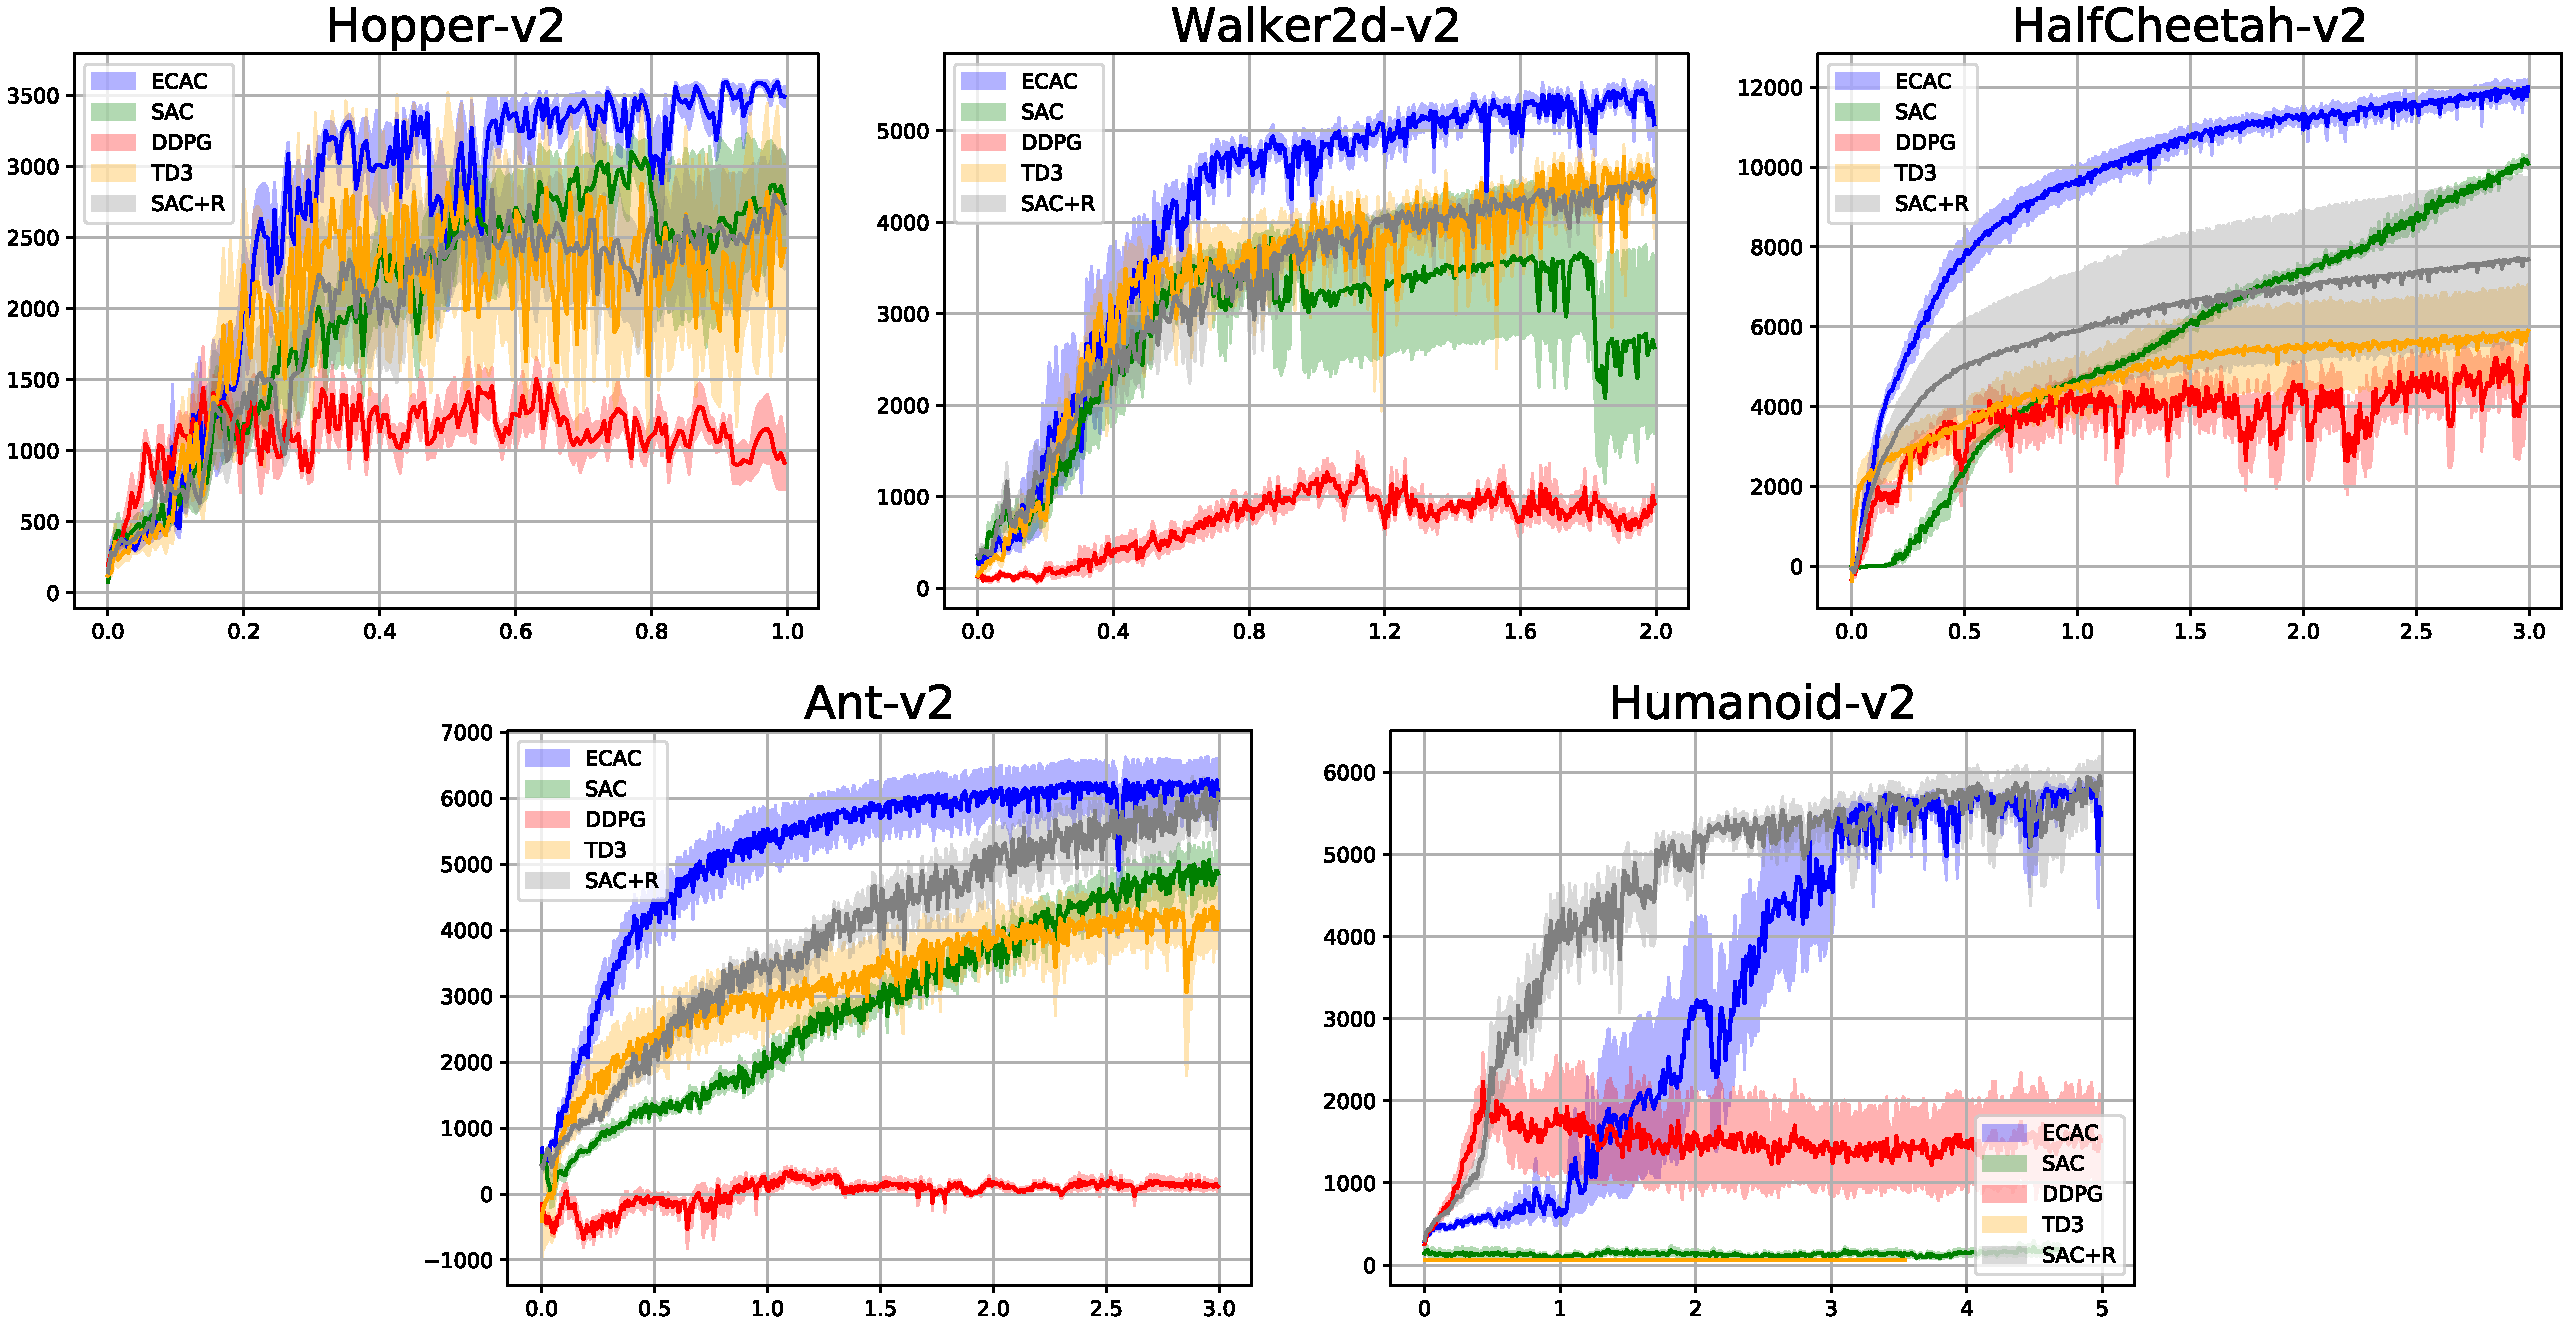
\includegraphics[width=0.7\linewidth]{./mujoco-results.pdf}
\end{center}
\caption{
Learning curves of DDPG (red), TD3 (yellow), SAC (green) and ECAC (blue) on
Mujoco tasks (with SAC+R (gray) added on Humanoid).
Plots show mean reward with standard error during training,
averaged over five different instances with different random seeds.
X-axis is millions of environment steps.
%We observe that ECAC is consistently able to match and, in many cases,
%the performance of the baseline algorithms across all tasks,
%both in terms of final performance and sample efficiency;
%the sole exception being SAC+R on Humanoid.
}
\label{fig:result-mujoco} 
\end{figure*}

\cref{fig:result-mujoco} presents the 
continuous control benchmarks, reporting the mean returns
on evaluation rollouts obtained by the algorithms during learning.
The
results are averaged over five instances
with different random seeds.
The solid curves corresponds to the mean and the shaded region to the
standard errors over the five trials.
\if0
To ensure a fair comparison with ECAC, we implemented the double-Q
but not the reparameterization trick for SAC 
(see equation (11)-(13) in \citep{haarnoja2018soft}).
This difference explains the discrepancy between the results we see here
and those reported in \citep{haarnoja2018soft}.
\fi
We observe that the reparameterization trick dramatically improve the performance of SAC. 
Therefore, to gain further clarity, 
we also report the result of SAC with the reparameterization trick,
denoted SAC+R.
%on Humanoid using the author's GitHub implementation.
The results show that ECAC matches or, in many cases, surpasses all other
baseline algorithms in both final performance and sample efficiency across
tasks, except compared to SAC+R in Humanoid.
In Humanoid, although SAC+R outperforms ECAC,
its final performance is still comparable with SAC+R.

%\begin{wrapfigure}{R}{0.5\textwidth}
%\label{fig:ablation}
%  \begin{center}
%    \includegraphics[width=0.5\textwidth]{Copy.png}
%  \end{center}
%  \caption{Hello, Bye!}
%\end{wrapfigure}

\subsection{Ablation Study}
\label{subsec:ablationstudy}

The comparative evaluations provided before suggest 
that our proposed algorithms 
%based on the policy optimization method \ref{eq:ECPO} 
outperform conventional RL methods on a number of challenging benchmarks.
In this section, we further investigate how each novel component of
\cref{eq:ECPO} improves learning performance,
by performing an ablation study on ReversedAddition and Ant. The results are presented in \cref{fig:ablation},
which clearly indicate all of the three major components of \cref{eq:ECPO}
are helpful for achieving better performance. 

%\piccaption[]{Ablation Study.\label{fig:ablation}}
%\parpic[r]{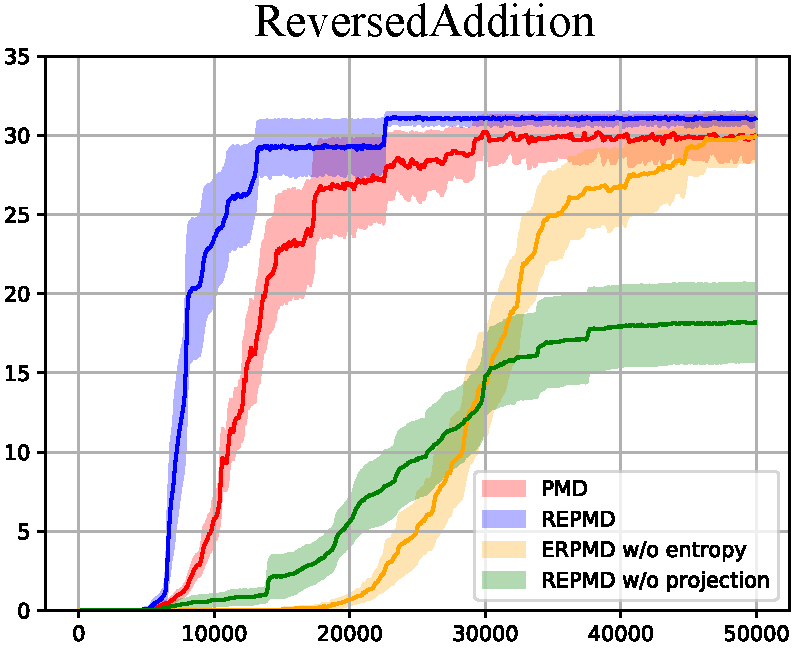
\includegraphics[width=0.35\linewidth]{ablation.pdf}}

\paragraph{Importance of entropy regularizer.} The main difference between the objective in \cref{eq:ECPO} and the PMD
objective \cref{eq:pmd} is the entropy regularizer.
We demonstrate the importance of this choice by presenting the results of ECPO and ECAC without the extra entropy regularizer, i.e. $\tau'=0$.

\paragraph{Importance of KL divergence projection.} Another important difference between \cref{eq:ECPO} with other RL methods
is to use a Project Step to update the policy,
rather than one SGD.
To show the importance of the Project Step,
we test ECPO and ECAC without projection,
which only performs one step of gradient update at each iteration of training. 

\paragraph{Importance of direction of KL divergence.} We choose PMD \cref{eq:pmd} as another baseline
to prove the effectiveness of using the \emph{mean seeking}
direction of KL divergence in the project step.
Similar to ECPO, we add a separate temperature parameter $\tau' > 0$
to the original objective function in \cref{eq:pmd}
to encourage policy exploration,
which gives
$\argmax_{\pi_\theta \in \Pi}{ \ep_{\rho \sim \pi_\theta}{  r(\rho)  - \tau \text{KL}(\pi_\theta \| \refPi) } + \tau'\cH(\pi_\theta) }$.
We name it PMD+entropy.
The corresponding algorithms in the actor-critic setting,
named PMD-AC and PMD-AC+entropy, are also implemented for comparison.

\begin{figure}[t]
\begin{center}
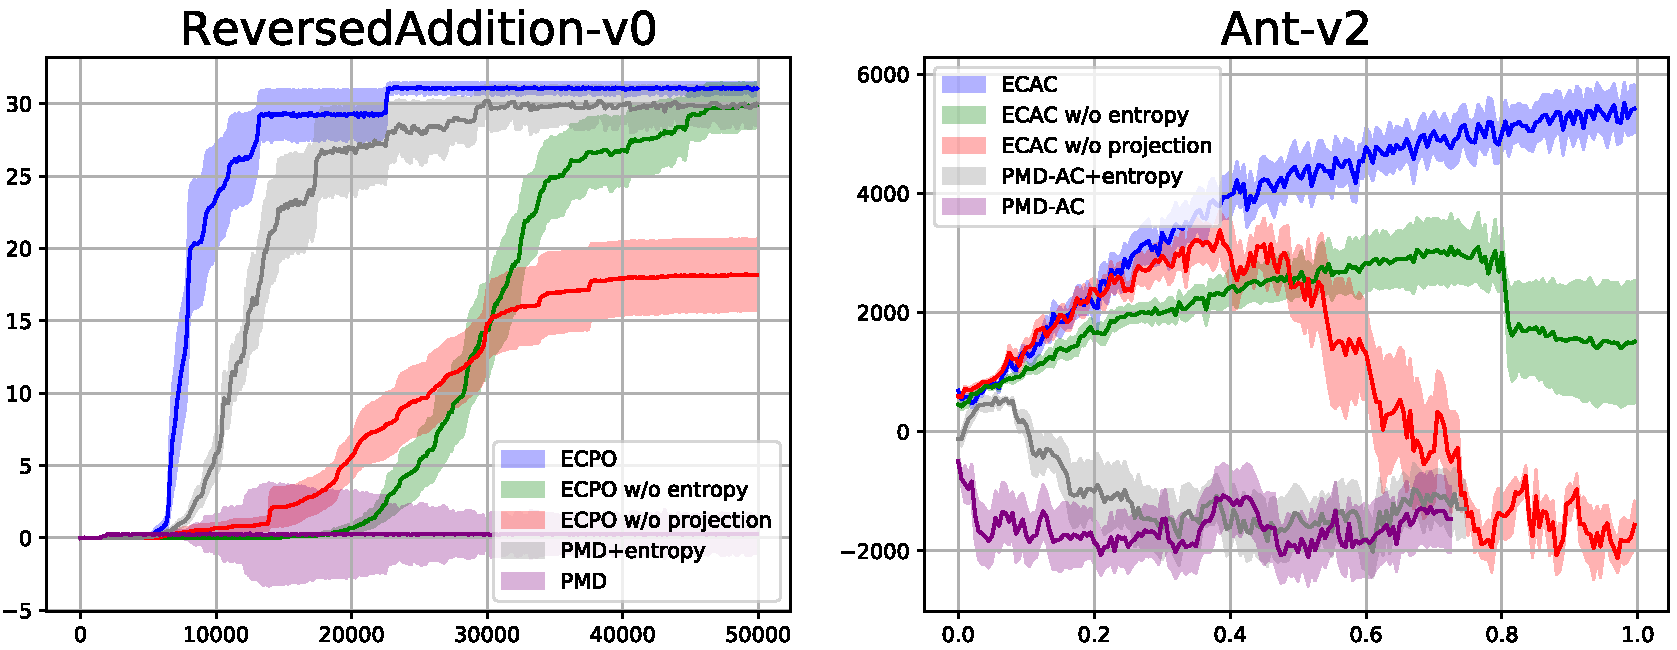
\includegraphics[width=0.9\linewidth]{./ablation-results.pdf}
\end{center}
\caption{Ablation Study of ECPO and ECAC. }
\label{fig:ablation}
\end{figure}

